\documentclass{article}
\usepackage[utf8]{inputenc}
\usepackage[margin=4cm]{geometry}

\usepackage{xcolor}
\usepackage{amsmath}
\usepackage{amssymb}
\usepackage{amsthm}
\usepackage{bbm}
\usepackage{enumitem}

\renewcommand{\arraystretch}{1.4}
\usepackage{xspace}
\newcommand{\seb}[1]{\xspace\textcolor{red}{#1 ---SB}\xspace} %% for comments

%%% MATHS ENVIRONMENTS
\usepackage[nobreak]{mdframed}
\newmdtheoremenv[backgroundcolor=gray!20, linewidth=0pt]{theorem}{Theorem}
\newmdtheoremenv[backgroundcolor=gray!20, linewidth=0pt]{corollary}[theorem]{Corollary}
\newmdtheoremenv[backgroundcolor=gray!20, linewidth=0pt]{prop}[theorem]{Proposition}
\newmdtheoremenv[backgroundcolor=gray!20, linewidth=0pt]{lemma}[theorem]{Lemma}
\theoremstyle{definition}
\newmdtheoremenv[backgroundcolor=gray!20, linewidth=0pt]{defn}[theorem]{Definition}
\renewcommand{\qedsymbol}{$\blacksquare$}

%%% MATHS COMMANDS
\newcommand{\Prob}{\mathbb{P}}
\newcommand{\E}{\mathbb{E}}
\newcommand{\Et}{\mathbb{E}_t}
\newcommand{\V}{\operatorname{Var}}
\newcommand{\Cov}{\operatorname{Cov}}
\newcommand{\ON}{1_N}
\newcommand{\eqdist}{\overset{d}{=}}
\newcommand{\I}[1]{\mathbbm{1}_{\{#1\}}}
\newcommand{\1}[1]{\mathbbm{1}_{#1}} % JK uses mathds{1} for indicators
\newcommand{\midd}{\,\middle|\,}        % for big conditional probability bar
\newcommand{\Mn}{\operatorname{Multinomial}}
\newcommand{\Bin}{\operatorname{Binomial}}
\newcommand{\Cat}{\operatorname{Categorical}}
\newcommand{\Exp}{\operatorname{Exp}}
\newcommand{\Unif}{\operatorname{Uniform}}
\newcommand{\Bern}{\operatorname{Bernoulli}}
\newcommand{\flnw}[1][i]{\lfloor N w_t^{(#1)} \rfloor}
\DeclareMathOperator*{\argmin}{argmin}
\DeclareMathOperator*{\argmax}{argmax}

%%% GRAPHICS
\usepackage{graphicx}
\usepackage{tikz}
\usetikzlibrary{decorations.pathreplacing}
\usepackage{subfig}

% custom header/footer
\usepackage{fancyhdr}
\pagestyle{fancy}
\renewcommand{\headrulewidth}{0pt}
\fancyhf{}
\rfoot{\textsf{\thepage}}
\lfoot{\textsf{Suzie Brown}}

%%% HYPERLINKS (must load last)
\usepackage{hyperref}

\title{Stratified resampling ++}
\author{Suzie Brown}
\date{21 May 2021}

\begin{document}
\maketitle
\thispagestyle{fancy}

\begin{enumerate}[label=(A\arabic*)]
\item\label{standing_assumption} The conditional distribution of parental indices $a_t^{(1:N)}$ given offspring counts $\nu_t^{(1:N)}$ is uniform over all assignments such that $ |\{ j: a_t^{(j)} =i \}|= \nu_t^{(i)} $ for all $i$.
%valid assignments.
\end{enumerate}



There are complex dependencies between the offspring counts, but we can still find some constraints on the distribution of each count conditional on the corresponding weight.
Write the $i^{th}$ weight in the form $w_t^{(i)} = (K + \delta)/N$, where $\delta \in [0,1)$ and $K\in \{0,\dots,N-1\}$.
The distribution of $\nu_t^{(i)}$ depends not only on $w_t^{(i)}$ but also on where the $i^{th}$ weight interval falls with respect to the length-$(1/N)$ intervals for inversion sampling. There are two cases to consider, which are illustrated in Figure~\ref{fig:strat_cases}. Note that Case \subref{fig:strat_case2} cannot happen if $K=0$.

%\begin{figure}
%\centering
%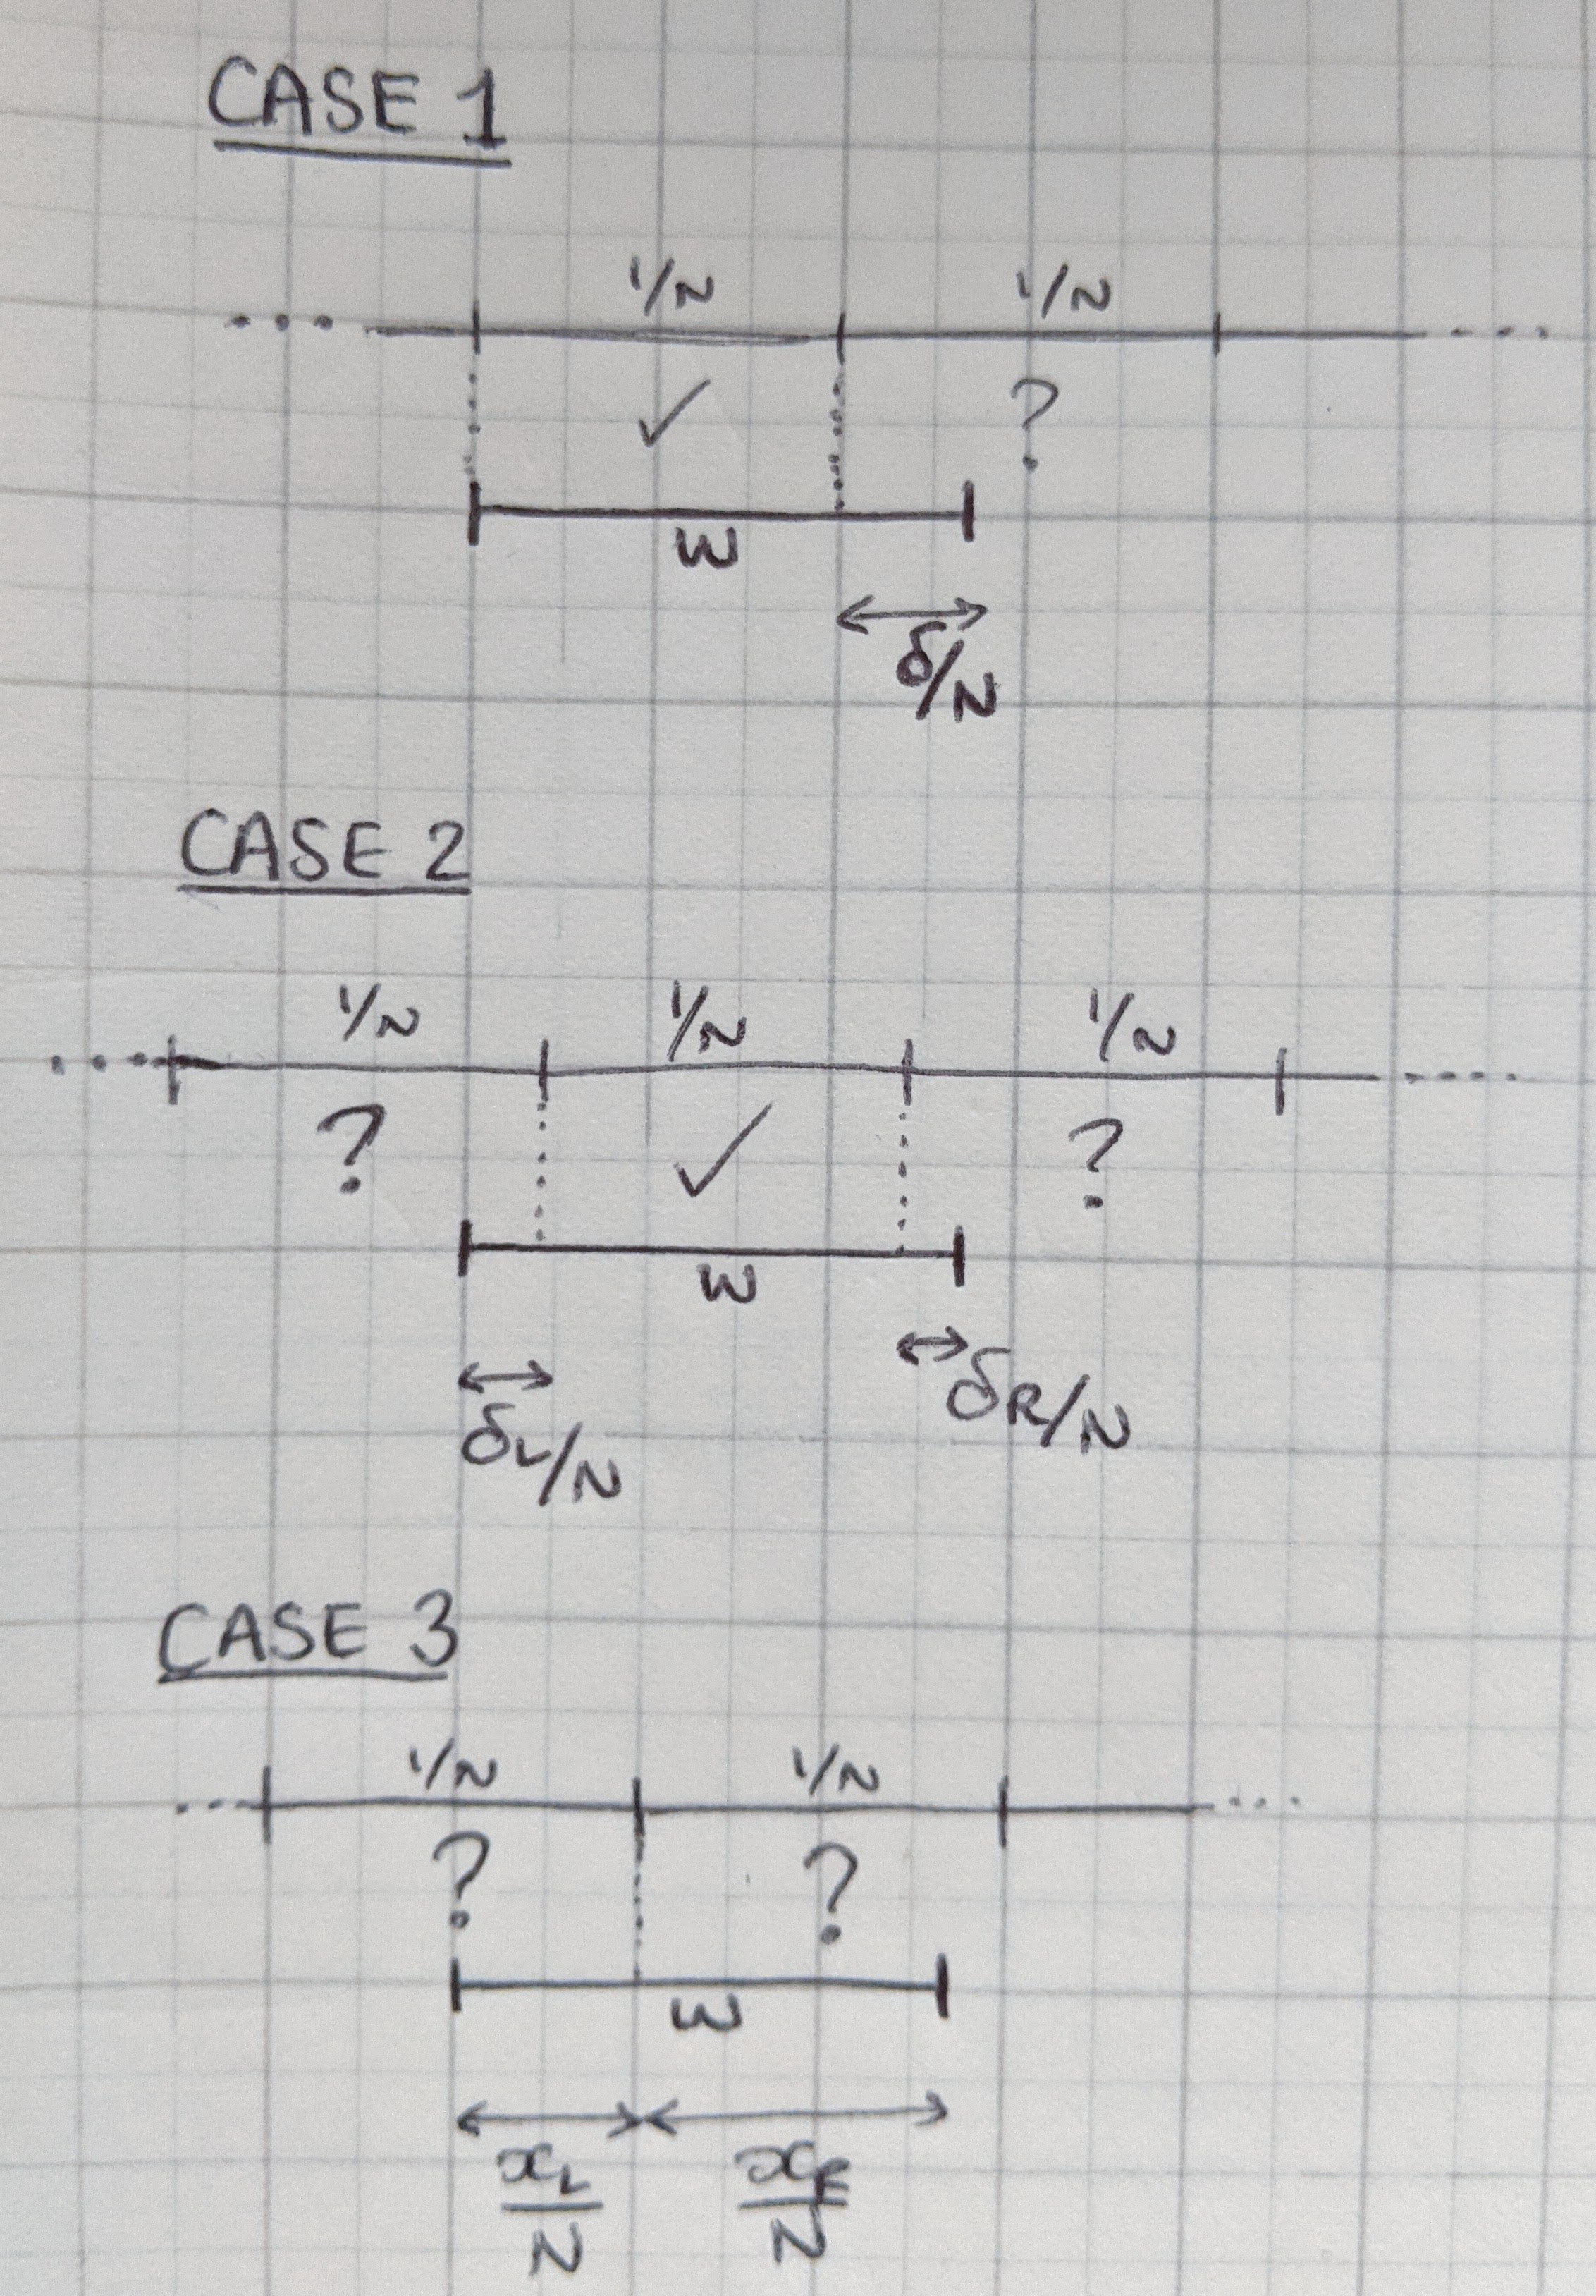
\includegraphics[width=0.4\textwidth]{plots/cases_sketch.jpg}
%\caption[PLACEHOLDER Cases for stratified resampling with a fixed weight]{PLACEHOLDER Cases for stratified resampling with a fixed weight. When I make this properly I need to allow for general $k$ rather than fixing $k=1$ as done here. Case 3 is only valid for $k\geq1$.}
%\label{fig:strat_cases_temp}
%\end{figure}

\begin{figure}
\centering
%\subfloat[Case 1]{
%\begin{tikzpicture}
%% w subinterval
%\draw[thick] (0,0)--(1.9,0);
%\draw[thick,dotted] (1.9,0)--(2.3,0);
%\draw[thick] (2.3,0)--(4.8,0);
%\draw[thick] (0,0.1)--(0,-0.1);
%\draw[thick] (4.8,0.1)--(4.8,-0.1);
%\node[anchor=north] at (2.4,0) {$w$};
%% length labels
%\draw[<->] (0,-0.4)--(4,-0.4);
%\node[anchor=north] at (2,-0.4) {$k/N$};
%\draw[<->] (4,-0.4)--(4.8,-0.4);
%\node[anchor=north] at (4.4,-0.4) {$\delta/N$};
%% sampling interval
%\draw (-0.5,1.5)--(8.5,1.5);
%\draw[dotted] (-1,1.5)--(-0.5,1.5);
%\draw[dotted] (8.5,1.5)--(9,1.5);
%\draw (0,1.6)--(0,1.4);
%\draw (4,1.6)--(4,1.4);
%\draw (8,1.6)--(8,1.4);
%\node[anchor=south] at (2,1.5) {$k/N$};
%\node[anchor=south] at (6,1.5) {$1/N$};
%% vertical dividers
%\draw[dashed, gray] (0,1.4)--(0,0.1);
%\draw[dashed, gray] (4,1.4)--(4,0.1);
%\end{tikzpicture}
%}\\
\subfloat[The parent under consideration is automatically assigned $K$ offspring, plus up to two more. ($\delta_L+\delta_R=\delta$.) ]{ %\delta_L, \delta_R \in [0,\delta]. 
\begin{tikzpicture}
% w subinterval
\draw[thick] (0,0)--(1.9,0);
\draw[thick,dotted] (1.9,0)--(2.3,0);
\draw[thick] (2.3,0)--(4.8,0);
\draw[thick] (0,0.1)--(0,-0.1);
\draw[thick] (4.8,0.1)--(4.8,-0.1);
\node[anchor=north] at (2.4,0) {$w$};
% length labels
\draw[<->] (0.3,-0.4)--(4.3,-0.4);
\node[anchor=north] at (2,-0.4) {$k/N$};
\draw[<->] (4.3,-0.4)--(4.8,-0.4);
\node[anchor=north] at (4.55,-0.4) {$\delta_R/N$};
\draw[<->] (0,-0.4)--(0.3,-0.4);
\node[anchor=north] at (0.15,-0.4) {$\delta_L/N$};
% sampling interval
\draw (-4.2,1.5)--(8.8,1.5);
\draw[dotted] (-4.7,1.5)--(-4.2,1.5);
\draw[dotted] (8.8,1.5)--(9.3,1.5);
\draw (-3.7,1.6)--(-3.7,1.4);
\draw (0.3,1.6)--(0.3,1.4);
\draw (4.3,1.6)--(4.3,1.4);
\draw (8.3,1.6)--(8.3,1.4);
\node[anchor=south] at (-1.7,1.5) {$1/N$};
\node[anchor=south] at (2.3,1.5) {$K/N$};
\node[anchor=south] at (6.3,1.5) {$1/N$};
% vertical dividers
\draw[dashed, gray] (0.3,1.4)--(0.3,0.1);
\draw[dashed, gray] (4.3,1.4)--(4.3,0.1);
\end{tikzpicture}
\label{fig:strat_case1}
}\\
\subfloat[This case can only occur when $K\geq1$. The parent under consideration is automatically assigned $K-1$ offspring, plus up to two more. ($x_L+x_R=1+\delta$.)]{ %$x_L,x_R \in [\delta,1] $. 
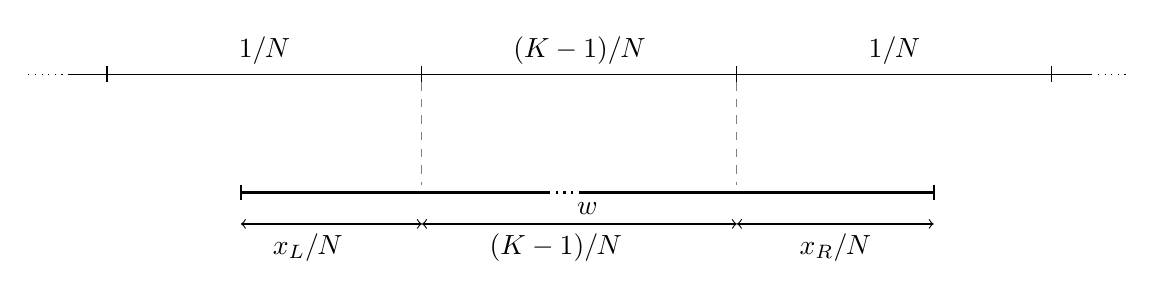
\begin{tikzpicture}
% w subinterval
\draw[thick] (-2,0)--(1.9,0);
\draw[thick,dotted] (1.9,0)--(2.3,0);
\draw[thick] (2.3,0)--(6.8,0);
\draw[thick] (-2,0.1)--(-2,-0.1);
\draw[thick] (6.8,0.1)--(6.8,-0.1);
\node[anchor=north] at (2.4,0) {$w$};
% length labels
\draw[<->] (0.3,-0.4)--(4.3,-0.4);
\node[anchor=north] at (2,-0.4) {$(K-1)/N$};
\draw[<->] (4.3,-0.4)--(6.8,-0.4);
\node[anchor=north] at (5.55,-0.4) {$x_R/N$};
\draw[<->] (-2,-0.4)--(0.3,-0.4);
\node[anchor=north] at (-1.15,-0.4) {$x_L/N$};
% sampling interval
\draw (-4.2,1.5)--(8.8,1.5);
\draw[dotted] (-4.7,1.5)--(-4.2,1.5);
\draw[dotted] (8.8,1.5)--(9.3,1.5);
\draw (-3.7,1.6)--(-3.7,1.4);
\draw (0.3,1.6)--(0.3,1.4);
\draw (4.3,1.6)--(4.3,1.4);
\draw (8.3,1.6)--(8.3,1.4);
\node[anchor=south] at (-1.7,1.5) {$1/N$};
\node[anchor=south] at (2.3,1.5) {$(K-1)/N$};
\node[anchor=south] at (6.3,1.5) {$1/N$};
% vertical dividers
\draw[dashed, gray] (0.3,1.4)--(0.3,0.1);
\draw[dashed, gray] (4.3,1.4)--(4.3,0.1);
\end{tikzpicture}
\label{fig:strat_case2}
}
\caption[Cases for stratified resampling with a fixed weight]{Cases for stratified resampling with a fixed weight $w = (K+\delta)/N$}
\label{fig:strat_cases}
\end{figure}


In any case $\nu_t^{(i)} \in \{k-1,k,k+1,k+2\}$ almost surely. 
To define a probability distribution over these four values, we introduce the notation $p_j := \Prob[ \nu_t^{(i)} = \flnw +j \mid w_t^{(i)} ]$, for $j=-1,0,1,2$. 
Since the sample within each interval of length $1/N$ is uniform over that interval, we find the probabilities given in Table~\ref{tab:strat_probs}, in terms of $\delta$ and the other quantities $\delta_L, \delta_R \in [0, \delta]$ and $x_L, x_R \in [\delta,1]$ defined in Figure~\ref{fig:strat_cases}. The probabilities do not depend on $k$, but of course the corresponding values of $\nu_t^{(i)}$ do. By definition $\delta_L+\delta_R=\delta$ and $x_L+x_R=1+\delta$.

\begin{table}[ht]
\centering
\begin{tabular}{ c | c c | c c }
& Case \subref{fig:strat_case1} & Case \subref{fig:strat_case2} & L.B. & U.B. \\
\hline
$p_{-1}$ & 0 & $x_Lx_R-\delta$ & 0 & $1/4$ \\
$p_0$ & $1-\delta + \delta_L\delta_R$ & $1+\delta-2x_Lx_R$ & $(1-\delta)^2 /2$ 
        & $1 - 3\delta /4$ \\
$p_1$ & $\delta-2\delta_L\delta_R$ & $x_Lx_R$ & $\delta /2$ & $(1+\delta)/2$ \\
$p_2$ & $\delta_L\delta_R$ & 0 & 0 & $1/4$ \\
\end{tabular}
\caption[Analysis of distribution of offspring counts under stratified resampling]{Marginal probability distribution of $\nu_t^{(i)}$ conditional on $w_t^{(i)}$, in terms of $\delta$ and the quantities defined in Figure~\ref{fig:strat_cases}, along with upper and lower bounds on these in terms of $\delta$ only, which hold in both cases i.e.\ whenever $w_t^{(i)} = (K+\delta)/N$.}
\label{tab:strat_probs}
\end{table}




\begin{theorem}\label{thm:FDDconv}
Let $\nu_t^{(1:N)}$ denote the offspring numbers in an interacting particle system satisfying \ref{standing_assumption} such that, for any $N$ sufficiently large, $\Prob[ \tau_N(t) = \infty ] =0$ for all finite $t$. Suppose that there exists a deterministic sequence $(b_N)_{N\geq1}$ such that ${\lim}_{N\to\infty} b_N =0$ and
\begin{equation}\label{eq:mainthmcond}
\frac{1}{(N)_3} \sum_{i = 1}^N \Et[ (\nu_t^{(i)})_3 ]  \leq b_N \frac{1}{(N)_2} \sum_{i = 1}^N \Et[ (\nu_t^{(i)})_2 ]
\end{equation}
for all $N$, uniformly in $t \geq 1$.
Fix $n\leq N$ and consider a randomly chosen sample of $n$ terminal particles.
Then the resulting rescaled genealogical process $(G_{\tau_N(t)}^{(n,N)})_{t\geq0}$ converges in the sense of finite-dimensional distributions to Kingman's $n$-coalescent as $N \to \infty$.
\end{theorem}

\begin{corollary}\label{thm:stratified}
Consider an SMC algorithm using stratified resampling, such that \ref{standing_assumption} is satisfied.
Assume that there exists a constant $a\in [1,\infty)$ such that for all $x, x^\prime, t$,
\begin{equation}\label{eq:gq_bounds_sr}
\frac{1}{a} \leq g_t(x, x^\prime) \leq a .
\end{equation}
Assume that $\Prob[ \tau_N(t) = \infty] =0$ for all finite $t$.
Let $(G_t^{(n,N)})_{t\geq0}$ denote the genealogy of a random sample of $n$ terminal particles from the output of the algorithm when the total number of particles used is $N$. Then, for any fixed $n$, the time-scaled genealogy $(G_{\tau_N(t)}^{(n,N)})_{t\geq0}$ converges to Kingman's $n$-coalescent as $N\to \infty$, in the sense of finite-dimensional distributions.
\end{corollary}

\begin{proof}
Recall that the sequence of $\sigma$-algebras
\begin{equation}\label{eq:defn_Ht}
\mathcal{H}_t := \sigma(X_{t-1}^{(1:N)}, X_t^{(1:N)}, w_{t-1}^{(1:N)}, w_t^{(1:N)} )
\end{equation}
are such that $\nu_t^{(1:N)}$ is conditionally independent of the filtration $\mathcal{F}_{t-1}$ given $\mathcal{H}_t$.
With stratified resampling, conditional on the weights each offspring count almost surely takes one of four values: $\nu_t^{(i)} \in \{ \flnw -1, \flnw, \flnw +1, \flnw +2 \}$.  
Denote $p_j^{(i)} := \Prob[ \nu_t^{(i)} = \flnw +j \mid \mathcal{H}_t ]$ for $j=-1,0,1,2$.
Now
\begin{align*}
\E [(\nu_t^{(i)})_2 \mid \mathcal{H}_t ]
&= p_{-1}^{(i)} (\flnw -1)_2 + p_0^{(i)} (\flnw)_2 + p_1^{(i)} (\flnw +1)_2 \\
    &\hspace{3cm} + p_2^{(i)} (\flnw +2)_2
\end{align*}
and
\begin{align*}
\E [(\nu_t^{(i)})_3 \mid \mathcal{H}_t ]
&= p_{-1}^{(i)} (\flnw -1)_3 + p_0^{(i)} (\flnw)_3 + p_1^{(i)} (\flnw +1)_3 \\
    &\hspace{1cm} + p_2^{(i)} (\flnw +2)_3 \\
&= p_{-1}^{(i)} (\flnw -3)(\flnw -1)_2 + p_0^{(i)} (\flnw -2)(\flnw)_2 \\
     &\hspace{1cm} + p_1^{(i)} (\flnw -1)(\flnw +1)_2 
         + p_2^{(i)} \flnw (\flnw +2)_2 \\
&\leq \flnw \{ p_0^{(i)} (\flnw)_2 + p_1^{(i)} (\flnw +1)_2 \} \\
&= \flnw ]\E [(\nu_t^{(i)})_2 \mid \mathcal{H}_t ] \\
&\leq a^2 \E [(\nu_t^{(i)})_2 \mid \mathcal{H}_t ]
\end{align*}
The last line uses the almost sure bound $w_t^{(i)} \leq a^2 /N$ which follows from \eqref{eq:gq_bounds_sr} along with the form of the weights in Algorithm \ref{alg:SMC}.
Note that some terms in the above expressions may be equal to zero when $w_t^{(i)}$ is small enough, but the bound always holds nonetheless.
Since the above holds for all $i$, applying the tower rule we have
\begin{equation*}
\frac{1}{(N)_3} \sum_{i=1}^{N} \Et [(\nu_t^{(i)})_3 ]
\leq \frac{a^2}{N-2} \frac{1}{(N)_2} \sum_{i=1}^{N} \Et [(\nu_t^{(i)})_2 ]
\end{equation*}
satisfying \eqref{eq:mainthmcond} with $b_N := a^2/(N-2) \rightarrow 0$.
The result then follows by applying Theorem~\ref{thm:FDDconv}.
\end{proof}



\begin{lemma}\label{thm:strat_nontriviality}
Consider an SMC algorithm using stratified resampling.
Suppose that 
\begin{equation*}
\varepsilon \leq q_t(x, x^\prime) \leq \varepsilon^{-1}
\end{equation*}
uniformly in $x,x^\prime$ for some $\varepsilon \in (0,1]$, and that there exist $\zeta >0$ and $\delta \in (0,1)$ such that 
\begin{equation*}
\Prob[ \max_i w_t^{(i)} - \min_i w_t^{(i)} \geq 2\delta/N \mid \mathcal{F}_{t-1} ] \geq \zeta
\end{equation*}
 for infinitely many $t$. Then, for all $N>1$, $\Prob[ \tau_N(t) = \infty ] =0$ for all finite $t$.
\end{lemma}


\begin{proof}
It is sufficient \seb{by a Borel-Cantelli argument, which is written somewhere else} to prove that under the stated conditions
\begin{equation*}
\sum_{r=0}^\infty \Prob[ c_N(r) > 2/N^2  \mid \mathcal{F}_{r-1} ] = \infty .
\end{equation*}
Firstly,
\begin{align}
\Prob[ c_N(t) \leq 2/N^2 \mid \mathcal{H}_t ]
&= \Prob[ c_N(t) =0 \mid \mathcal{H}_t ]
= \Prob[ \nu_t^{(i)} =1 \,\forall i\in\{1,\dots,N\} \mid \mathcal{H}_t ] \notag\\
&\leq \Prob[ \nu_t^{(i^\star)} =1 \mid \mathcal{H}_t ] , \label{eq:cNnonzero}
\end{align}
where $i^\star := \argmax_i \{ w_t^{(i)} \}$ (but note that the inequality holds when $i^\star$ is taken to be any particular index).
Define for any $k\in\mathbb{Z}$
\begin{equation*}
p_k^{(i)} := \Prob \left[ \nu_t^{(i)} = \flnw + k \midd \mathcal{H}_t \right] .
\end{equation*}
Since stratified resampling almost surely results in $\nu_t^{(i)} \in \{ \flnw-1, \flnw, \flnw+1, \flnw+2 \}$ we have that $p_k^{(i)} \equiv 0$ for $k\notin \{-1,0,1,2\}$, and
\begin{equation*}
\sum_{k=-1}^2 p_k^{(i)} 
= \sum_{k=-1}^2 \Prob \left[ \nu_t^{(i)} = \flnw + k \midd w_t^{(1:N)} \right]
= 1 .
\end{equation*}
Up to a proportionality constant $C$,
\begin{align*}
p_k^{(i)} 
&= C \, \Prob \left[ \nu_t^{(i)} = \flnw + k \midd w_t^{(1:N)} \right] \\
    &\qquad \times \sum_{\substack{a_{1:N} \in \{1,\dots,N\}^N : 
        \\ |\{j: a_j=i\}|=\flnw +k }}
        \Prob\left[ a_t^{(1:N)} = a_{1:N} \midd \nu_t^{(i)}, w_t^{(1:N)} \right]
        \prod_{j=1}^N q_{t-1}( X_t^{(a_j)}, X_{t-1}^{(j)} ) 
\end{align*}
for each $k\in\{-1,0,1,2\}$.
We can bound each probability above and below using the almost sure bounds on $q_{t-1}$ stated in the Lemma:
\begin{equation*}
C \, \Prob \left[ \nu_t^{(i)} = \flnw + k \midd w_t^{(1:N)} \right] \varepsilon^N
\leq p_k^{(i)}
\leq C \, \Prob \left[ \nu_t^{(i)} = \flnw + k \midd w_t^{(1:N)} \right] \varepsilon^{-N}
\end{equation*}
then eliminate the constant $C$ by normalising, to obtain lower bounds
\begin{align}
p_k^{(i)} 
&\geq \frac{ C \, \Prob [ \nu_t^{(i)} = \flnw + k \mid w_t^{(1:N)} ] \varepsilon^N }{
        \sum_{j=-1}^2 C \, \Prob [ \nu_t^{(i)} = \flnw + j \mid w_t^{(1:N)} ] 
        \varepsilon^{-N} } \notag\\
%&= \frac{ \Prob [ \nu_t^{(i)} = \flnw + k \mid w_t^{(1:N)} ] \varepsilon^N }{
%        \varepsilon^{-N} } \notag\\
&= \Prob [ \nu_t^{(i)} = \flnw + k \mid w_t^{(1:N)} ] \varepsilon^{2N} 
        . \label{eq:strat_pbounds}
\end{align}

Suppose that $\max_i w_t^{(i)} - \min_i w_t^{(i)} \geq 2\delta/N$. Then that at least one of $\{ \max_i w_t^{(i)} \geq (1+\delta)/N \}$ and $\{ \min_i w_t^{(i)} \leq (1-\delta)/N \}$ occurs. We will now examine each of these possibilities.

We can always write the maximum weight as $w_t^{(i^\star)} = \frac{1+\gamma}{N}$ for some $\gamma \geq 0$. Then, using \eqref{eq:cNnonzero},
\begin{equation*}
\Prob[ c_N(t) > 2/N^2 \mid \mathcal{H}_t ]
\geq 1- \Prob[ \nu_t^{(i^\star)} =1 \mid \mathcal{H}_t ]
= \begin{cases}
    0 & \text{if } \gamma = 0 \\
    1 - p_0^{(i^\star)} & \text{if } \gamma \in (0,1) \\
    1 - p_{-1}^{(i^\star)} & \text{if } \gamma \in [1,2) \\
    1 & \text{if } \gamma \geq 2 .
\end{cases}
\end{equation*}
If $\gamma \in (0,1)$ then
%\begin{equation*}
%1 - p_0^{(i^\star)}
%= p_{-1}^{(i^\star)} + p_1^{(i^\star)} + p_2^{(i^\star)}
%\geq \left( 0 + \frac{\delta^\prime}{2} + 0 \right) \varepsilon^{2N} 
%= \frac{\delta^\prime \varepsilon^{2N} }{2}
%\end{equation*}
\begin{equation*}
1 - p_0^{(i^\star)}
%\geq 1 - \left( 1- \frac{3\delta^\prime}{4} \right) \varepsilon^{2N} 
\geq \frac{3\gamma \varepsilon^{2N} }{4}
\end{equation*}
using \eqref{eq:strat_pbounds} and %the lower bounds in 
Table~\ref{tab:strat_probs} ($p_0$, U.B.).
Similarly, if $\gamma \in [1,2)$ then by Table~\ref{tab:strat_probs} ($p_{-1}$, U.B.),
%\begin{equation*}
%1 - p_{-1}^{(i^\star)}
%= p_0^{(i^\star)} + p_1^{(i^\star)} + p_2^{(i^\star)}
%\geq \left( \frac{(1-\delta^\prime)^2}{2} + \frac{\delta^\prime}{2} + 0 \right)
%        \varepsilon^{2N} 
%\geq \frac{\delta^\prime \varepsilon^{2N} }{2} .
%\end{equation*}
\begin{equation*}
1 - p_{-1}^{(i^\star)}
\geq \left( 1- \frac{1}{4} \right)
        \varepsilon^{2N} 
\geq \frac{3 \varepsilon^{2N} }{4} .
\end{equation*}
So overall, under the constraint $\max_i w_t^{(i)} \geq (1+\delta)/N$, we have
%\begin{equation*}
%\Prob[ c_N(t) > 2/N^2 \mid \mathcal{H}_t ]
%\geq \min_{\delta^\prime \geq \delta} 
%        \left\{ \frac{\delta^\prime \varepsilon^{2N} }{2} \right\}
%= \frac{ \delta \varepsilon^{2N} }{2} .
%\end{equation*}
\begin{equation*}
\Prob[ c_N(t) > 2/N^2 \mid \mathcal{H}_t ]
\geq \min_{\gamma \geq \delta} 
        \left\{ \frac{3\gamma \varepsilon^{2N} }{4}\I{\gamma \in [0,1)}
        + \frac{3 \varepsilon^{2N} }{4}\I{\gamma \in [1,2)}
        + \I{\gamma \geq 2} \right\}
= \frac{ 3\delta \varepsilon^{2N} }{4} .
\end{equation*}

Now for the minimum weight. Let $j^\star := \argmin_i \{ w_t^{(i)} \}$ and write
$w_t^{(j^\star)} = \frac{1-\gamma}{N}$, for some $\gamma \in [0,1]$.
Then we have
\begin{equation*}
\Prob[ c_N(t) > 2/N^2 \mid \mathcal{H}_t ]
\geq 1- \Prob[ \nu_t^{(j^\star)} =1 \mid \mathcal{H}_t ]
=\begin{cases}
    1- p_1^{(j^\star)} & \text{if } \gamma \in (0,1] \\
    0 & \text{if } \gamma =0 .
\end{cases}
\end{equation*}
If $\gamma \in (0,1]$ then
%\begin{equation*}
%1- p_1^{(j^\star)} 
%= p_{-1}^{(j^\star)} + p_0^{(j^\star)} + p_2^{(j^\star)}
%\geq \left( 0 + \frac{ (\delta^\prime)^2 }{2} + 0 \right) \varepsilon^{2N}
%= \frac{ (\delta^\prime)^2 \varepsilon^{2N} }{2} ,
%\end{equation*}
\begin{equation*}
1- p_1^{(j^\star)}
\geq \left( 1- \frac{1+ (1-\gamma)}{2} \right) \varepsilon^{2N}
= \frac{ \gamma \varepsilon^{2N} }{2} ,
\end{equation*}
again using Table~\ref{tab:strat_probs} ($p_1$, U.B.).
Therefore, under the constraint $\min_i w_t^{(i)} \leq (1-\delta)/N$, we have
%\begin{equation*}
%\Prob[ c_N(t) > 2/N^2 \mid \mathcal{H}_t ]
%\geq \min_{\delta^\prime \geq \delta} 
%        \left\{ \frac{ (\delta^\prime)^2 \varepsilon^{2N} }{2} 
%        \I{\delta^\prime \neq 0} \right\}
%= \frac{ \delta^2 \varepsilon^{2N} }{2} .
%\end{equation*}
\begin{equation*}
\Prob[ c_N(t) > 2/N^2 \mid \mathcal{H}_t ]
\geq \min_{\gamma \geq \delta} 
        \left\{ \frac{ \gamma \varepsilon^{2N} }{2} 
        %\I{\gamma \neq 0}
        \right\}
= \frac{ \delta \varepsilon^{2N} }{2} .
\end{equation*}
Combining both cases, we find for arbitrary $r$
\begin{equation*}
\Prob[ c_N(r) > 2/N^2 \mid \mathcal{H}_r ] 
\geq  \frac{ \delta \varepsilon^{2N} }{2}
        \I{ \max_i w_r^{(i)} - \min_i w_r^{(i)} \geq 2\delta/N }
\end{equation*}
so
\begin{align*}
\Prob[ c_N(r) > 2/N^2 \mid \mathcal{F}_{r-1} ] 
&\geq  \frac{ \delta \varepsilon^{2N} }{2}
        \Prob[ \max_i w_r^{(i)} - \min_i w_r^{(i)} \geq 2\delta/N 
        \mid \mathcal{F}_{r-1} ] \\
&\geq \zeta \frac{ \delta \varepsilon^{2N} }{2}
> 0
\end{align*}
for infinitely many $r$.
Hence
\begin{equation*}
\sum_{r=0}^\infty \Prob[ c_N(r) > 2/N^2  \mid \mathcal{F}_{r-1} ] = \infty
\end{equation*}
as required.
\end{proof}



\end{document}